\documentclass{article}
\usepackage[margin=1in]{geometry}
\usepackage{amsmath,amsthm,amssymb}
\usepackage{bbm,enumerate,mathtools}
\usepackage{tikz,pgfplots}
\usepackage{chessboard}
\usepackage[hidelinks]{hyperref}
\usepackage{multicol} % Problem 35

\newenvironment{question}{\begin{trivlist}\item[\textbf{Question.}]}{\end{trivlist}}
\newenvironment{note}{\begin{trivlist}\item[\textbf{Note.}]}{\end{trivlist}}
\newenvironment{references}{\begin{trivlist}\item[\textbf{References.}]}{\end{trivlist}}
\newenvironment{related}{\begin{trivlist}\item[\textbf{Related.}]\end{trivlist}\begin{enumerate}}{\end{enumerate}}


\begin{document}
\rating{3}{3}
Consider all configurations of $n$ nonattacking rooks on an $n\times n$ board up
to dihedral action.
\begin{figure}[!h]
  \centering
  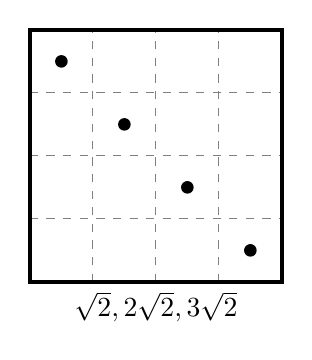
\begin{tikzpicture}[scale=0.8]
    % 1
    \draw[gray, dashed] (0,0) grid (4,4);
    \draw[ultra thick] (0,0) rectangle (4,4);
    \foreach \x/\y in {1/4,2/3,3/2,4/1} {
      \fill (\x - 0.5, \y - 0.5) circle (0.1cm);
    }
    \node at (2, -0.4) {$\sqrt{2}, 2\sqrt{2}, 3\sqrt{2}$};
  \end{tikzpicture}\hspace{1cm}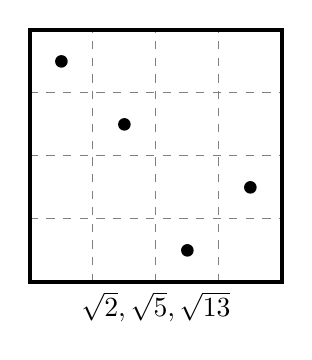
\begin{tikzpicture}[scale=0.8]
    % 2
    \draw[gray, dashed] (0,0) grid (4,4);
    \draw[ultra thick] (0,0) rectangle (4,4);
    \foreach \x/\y in {1/4,2/3,3/1,4/2} {
      \fill (\x - 0.5, \y - 0.5) circle (0.1cm);
    }
    \node at (2, -0.4) {$\sqrt{2}, \sqrt{5}, \sqrt{13}$};
  \end{tikzpicture}\hspace{1cm}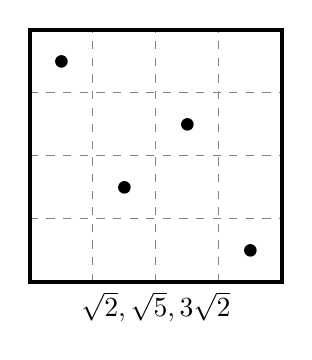
\begin{tikzpicture}[scale=0.8]
    % 3
    \draw[gray, dashed] (0,0) grid (4,4);
    \draw[ultra thick] (0,0) rectangle (4,4);
    \foreach \x/\y in {1/4,2/2,3/3,4/1} {
      \fill (\x - 0.5, \y - 0.5) circle (0.1cm);
    }
    \node at (2, -0.4) {$\sqrt{2}, \sqrt{5}, 3\sqrt{2}$};
  \end{tikzpicture}\hspace{1cm}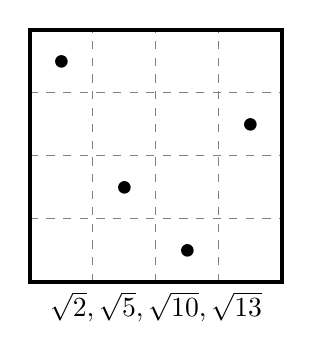
\begin{tikzpicture}[scale=0.8]
    % 4
    \draw[gray, dashed] (0,0) grid (4,4);
    \draw[ultra thick] (0,0) rectangle (4,4);
    \foreach \x/\y in {1/4,2/2,3/1,4/3} {
      \fill (\x - 0.5, \y - 0.5) circle (0.1cm);
    }
    \node at (2, -0.4) {$\sqrt{2}, \sqrt{5}, \sqrt{10}, \sqrt{13}$};
  \end{tikzpicture}\vspace{3mm}\\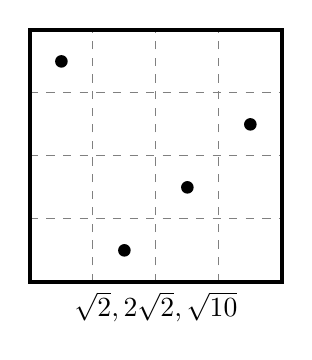
\begin{tikzpicture}[scale=0.8]
    % 5
    \draw[gray, dashed] (0,0) grid (4,4);
    \draw[ultra thick] (0,0) rectangle (4,4);
    \foreach \x/\y in {1/4,2/1,3/2,4/3} {
      \fill (\x - 0.5, \y - 0.5) circle (0.1cm);
    }
    \node at (2, -0.4) {$\sqrt{2}, 2\sqrt{2}, \sqrt{10}$};
  \end{tikzpicture}\hspace{1cm}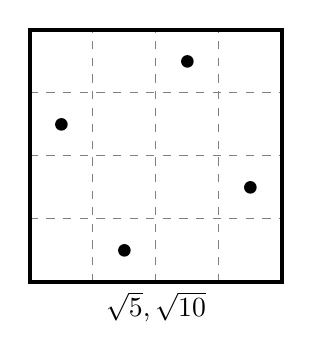
\begin{tikzpicture}[scale=0.8]
    % 6
    \draw[gray, dashed] (0,0) grid (4,4);
    \draw[ultra thick] (0,0) rectangle (4,4);
    \foreach \x/\y in {1/3,2/1,3/4,4/2} {
      \fill (\x - 0.5, \y - 0.5) circle (0.1cm);
    }
    \node at (2, -0.4) {$\sqrt{5}, \sqrt{10}$};
  \end{tikzpicture}\hspace{1cm}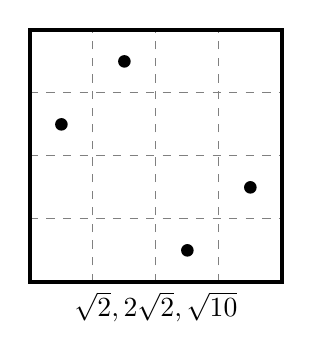
\begin{tikzpicture}[scale=0.8]
    % 7
    \draw[gray, dashed] (0,0) grid (4,4);
    \draw[ultra thick] (0,0) rectangle (4,4);
    \foreach \x/\y in {1/3,2/4,3/1,4/2} {
      \fill (\x - 0.5, \y - 0.5) circle (0.1cm);
    }
    \node at (2, -0.4) {$\sqrt{2}, 2\sqrt{2}, \sqrt{10}$};
  \end{tikzpicture}
  \caption{
    Each figure is marked with the distinct distances between pieces.
  }
\end{figure}

\begin{question}
  What is the minimum number of distinct distances on such a figure?
\end{question}
\begin{related}
  \item What is the minimum number of distinct directions on such a figure?
    (Directions up to dihedral action?)
  \item What if this is done with $n$ queens instead of rooks?
  \item What if this is done with $0 \leq k \leq n^2$ pieces, any of which are allowed
    to be in attacking positions?
  \item What if distance is measured by the taxicab metric? $d_3$? $d_\infty$?
  Number of knight-moves away? Number of king moves away?
  \item How many configurations of nonattacking rooks on the torus, rectangle,
  triangluar grid, and other geometries?
  \item Are any configurations of nonattacking rooks on the torus that can
    be meaningfully called a ``generalized Costas array''?
\end{related}
\begin{references}
  \item \url{https://en.wikipedia.org/wiki/Costas_array}
  \item The maximum and minimum number of distinct distances is given by
  A320448 and A319476 respectively.
  \item The number of extremal boards is given by
  A320573 and A320575 (A320574 and A320576, up to symmetry).
  \item A193838: smallest square pegboard from which $n$ points with distinct mutual distances can be chosen.
\end{references}
\end{document}
